\section{Overview and System Architecture}
The digital twin framework developed in this research requires a continuous, low-latency stream of sensor data to drive real-time predictive analytics across a manufacturing fleet of 50 heterogeneous machines. This section presents the data ingestion pipeline and the spatio-temporal modelling methodology underpinning the system. The architecture couples a physical Internet of Things (IoT) sensor layer—realised through a Plalion device measuring temperature, humidity, ozone, dust, CO₂, and volatile organic compounds (VOCs)—with a Temporal Graph Convolutional Network (T-GCN) that models the spatial dependencies and temporal dynamics across the machine fleet. The T-GCN framework, originally proposed by Zhao et al.\ \cite{Zhao2020} for traffic forecasting, is adapted here to the manufacturing domain, where machines exhibit non-trivial cross-correlation structures arising from shared production workflows, thermal coupling, and power-line transients. The end-to-end pipeline is illustrated in Figure \ref{fig:dt-sensors}.
\begin{figure}[!htbp]
    \centering
    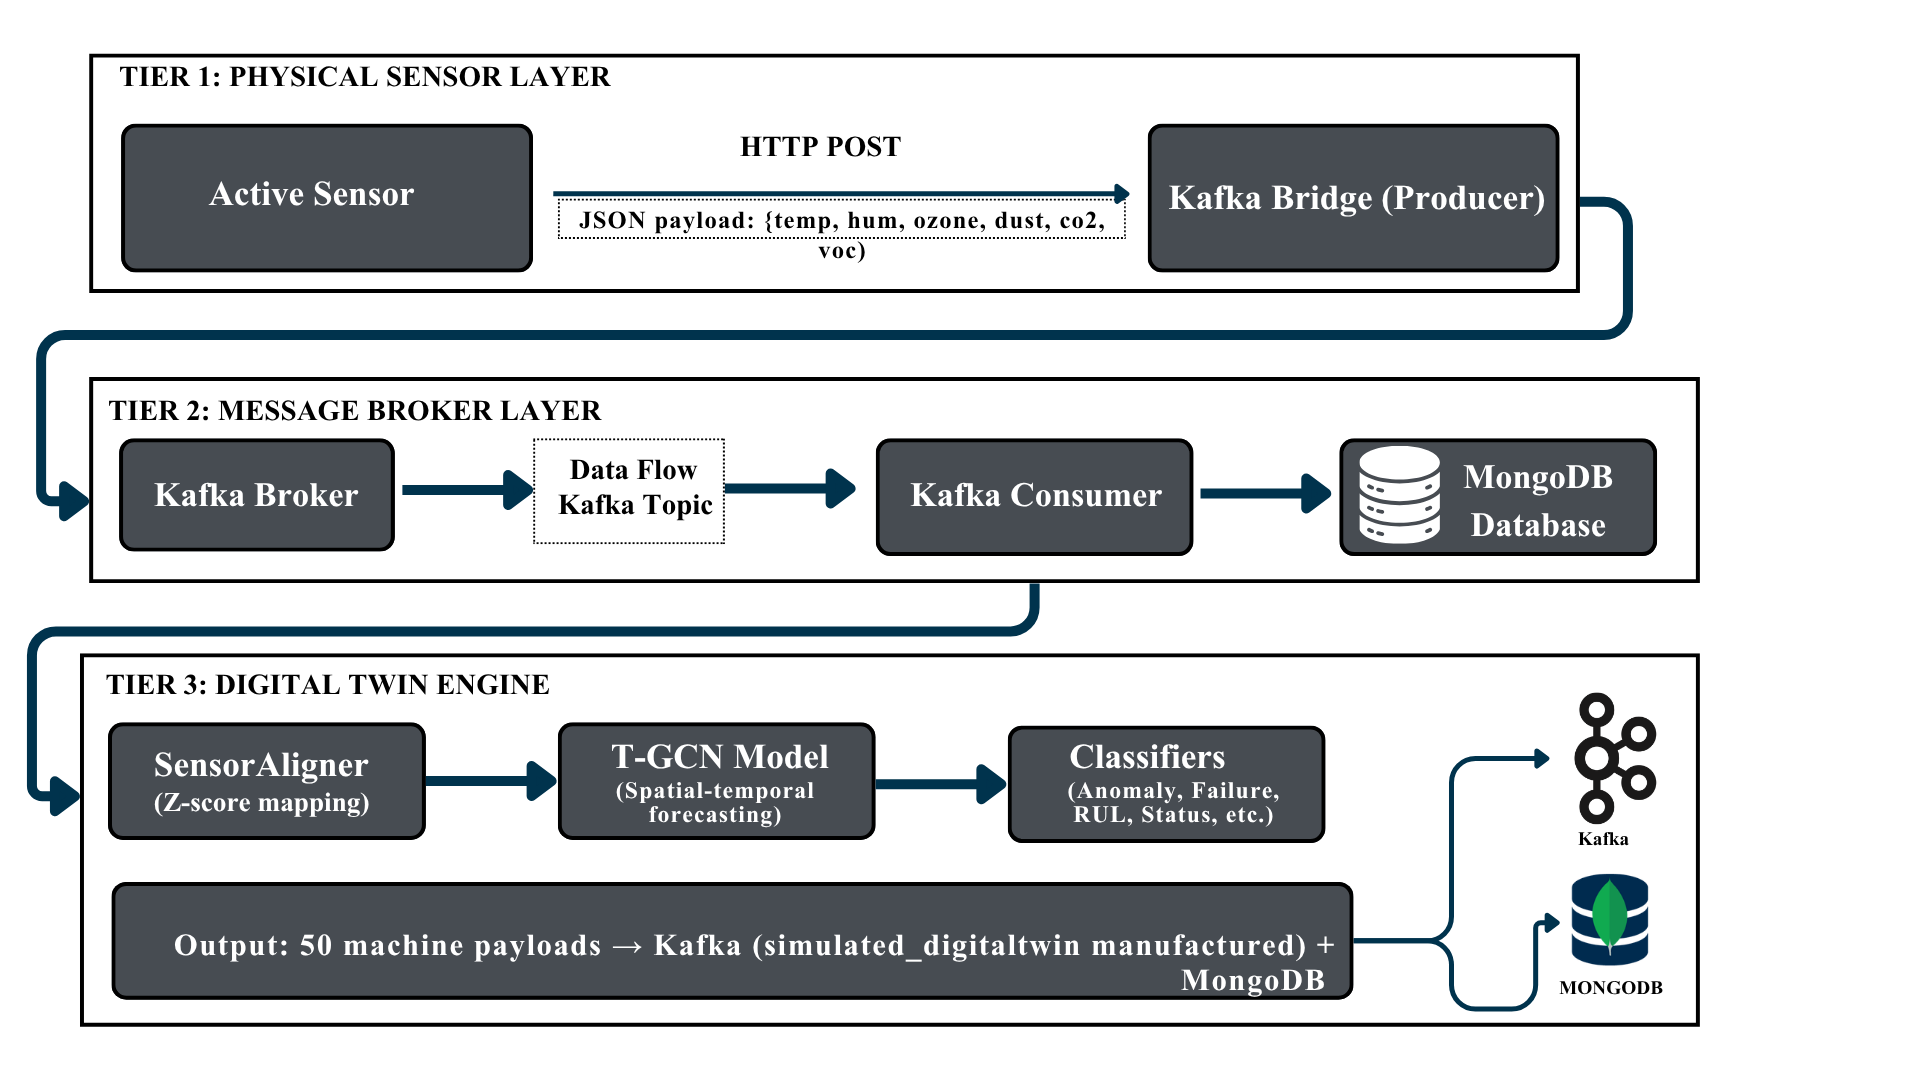
\includegraphics[width=1\textwidth]{figures/images/DT sensors.png}
    \caption{Three-tier system architecture for real-time data ingestion,
           spatio-temporal modelling, and state classification.}
    \label{fig:dt-sensors}
\end{figure}
The architecture is containerized using Docker and deployed on an Ubuntu 22.04 LTS operating system. Service orchestration utilities Docker Compose with a dedicated Kafka network, enabling inter-service communication without exposing internal ports. Each container is single-responsibility: the Plalion Kafka bridge exclusively handles device-to-broker relay, the consumer persists raw data into MongoDB, and the digital twin container encapsulates the entire modeling pipeline—from sensor alignment through fleet propagation and classification. This design supports modular scaling, fault isolation, and atomic deployment of model updates without disrupting the ingestion layer.

\section{Dataset Description and Sensor Characteristics}

Building on the dataset overview of Chapter~3 (\S3.3), this section reports the descriptive statistics that drive the modelling decisions of the forecasting layer; redundant enumeration of fields and basic correlations is omitted. The dataset is complete (no missing values across all $1{,}300{,}000$ data points), enabling unbroken sliding-window training without imputation.

Table~\ref{tab:sensor_stats} summarises the five continuous sensor channels. Two distributional properties drive forecasting-architecture choices. \emph{Vibration} shows a $19\%$ elevation in anomalous readings (mean $58.51$ vs $49.18$ normal) and is the primary indicator of the \texttt{Vibration Issue} failure type, motivating its first-difference treatment in the T-GCN input. \emph{Humidity} has near-zero linear correlation with the anomaly flag yet remains predictive through nonlinear cross-sensor interactions, supporting the inclusion of multi-channel feature engineering rather than per-channel modelling.

\begin{table}[!htbp]
\centering
\caption{Descriptive Statistics of Sensor Variables ($n = 100{,}000$)}
\label{tab:sensor_stats}
\small
\renewcommand{\arraystretch}{1.05}
\setlength{\tabcolsep}{5pt}
\begin{tabular}{lccccc}
\toprule
\textbf{Sensor} & \textbf{Min} & \textbf{Max} & \textbf{Mean} & \textbf{Std Dev} & \textbf{Corr.\ w/ Anomaly} \\
\midrule
Temperature (\textdegree C) & 35.55 & 121.94 & 75.02 & 10.03 & 0.447 \\
Vibration         & $-$17.09 & 113.80 & 50.42  & 14.31 & 0.198 \\
Humidity (\%)     & 30.00  & 80.00  & 55.01  & 10.00 & $\approx$ 0.001 \\
Pressure (bar)    & 1.00   & 5.00   & 3.00   & 1.15  & $\approx$ $-$0.002 \\
Energy (kWh)      & 0.50   & 5.00   & 2.75   & 1.30  & $\approx$ 0.006 \\
\bottomrule
\end{tabular}
\end{table}

Target-variable distributions (Table~\ref{tab:target_stats}) reflect the operational rarity of failure: $8.92\%$ anomaly positives, $9.85\%$ stopped + $10.06\%$ warning machine-statuses, severe failure-type imbalance ($91.90\%$ Normal vs four minority classes at $1$--$3\%$), and a near-uniform RUL distribution (mean $234$~h, std $150$~h). These properties drive the use of F1-score as the primary classification metric and motivate the supervised-benchmark design of \S4.7 below.

\begin{table}[!htbp]
\centering
\caption{Target Variable Distributions}
\label{tab:target_stats}
\small
\renewcommand{\arraystretch}{1.05}
\begin{tabular}{lccl}
\toprule
\textbf{Target Variable} & \textbf{Value / Class} & \textbf{Count} & \textbf{Percentage} \\
\midrule
Anomaly Flag         & Anomalous (1)            & 8,916  & 8.92\%  \\
                     & Normal (0)               & 91,084 & 91.08\% \\
\midrule
Machine Status       & Running (1)              & 80,091 & 80.09\% \\
                     & Warning (2)              & 10,057 & 10.06\% \\
                     & Stopped (0)              & 9,852  & 9.85\%  \\
\midrule
Failure Type         & Normal                   & 91,899 & 91.90\% \\
                     & Vibration Issue          & 3,129  & 3.13\%  \\
                     & Overheating              & 1,989  & 1.99\%  \\
                     & Pressure Drop            & 1,969  & 1.97\%  \\
                     & Electrical Fault         & 1,014  & 1.01\%  \\
\midrule
Downtime Risk        & High Risk ($= 1.0$)      & 8,904  & 8.90\%  \\
                     & No Risk ($= 0.0$)        & 91,084 & 91.08\% \\
\midrule
Maintenance Required & Required (1)             & 19,700 & 19.70\% \\
                     & Not Required (0)         & 80,300 & 80.30\% \\
\midrule
RUL (hours)          & Mean: 234.27 h           & Std: 150.06 h   & --- \\
                     & Critical ($< 50$ h)      & 16,333 & 16.33\% \\
                     & Imminent ($< 10$ h)      & 1,637  & 1.64\%  \\
\bottomrule
\end{tabular}
\end{table}

\section{Real-Time Sensor Data Ingestion}
Physical active sensor is performed by a environmental sensor, deployed within the manufacturing environment. The device exposes a REST API endpoint returning a JSON payload containing seven environmental parameters at a 10-second polling interval. The Kafka bridge, implemented as a Python producer container, executes the following loop:
\begin{algorithm}[!htbp]
\caption{Active Sensor to Kafka Ingestion Loop}
\label{alg:plalion_kafka}
\begin{algorithmic}[1]
\Require API\_URL, SERIAL\_NUMBER, KAFKA\_BOOTSTRAP, KAFKA\_TOPIC
\Ensure Continuous Kafka message stream
\State producer $\gets$ KafkaProducer(
\Statex \hspace{1.5em} bootstrap\_servers = KAFKA\_BOOTSTRAP,
\Statex \hspace{1.5em} acks = all,
\Statex \hspace{1.5em} retries = 3,
\Statex \hspace{1.5em} value\_serializer = JSON
\Statex )
\State message\_count $\gets$ 0
\While{true}
    \State payload $\gets$ \{ ``serial\_num'': SERIAL\_NUMBER \}
    \State response $\gets$ HTTP\_POST(API\_URL, payload, timeout = 10s)
    \If{response.status = 200}
        \State row $\gets$ response.json()[``rows''][0]
        \State kafka\_msg $\gets$ \{
        \Statex \hspace{2em} serial\_number, temp, hum, ozone,
        \Statex \hspace{2em} dust, co2, voc, timestamp
        \Statex \hspace{1em} \}
        \State future $\gets$ producer.send(
        \Statex \hspace{2em} KAFKA\_TOPIC,
        \Statex \hspace{2em} key = SERIAL\_NUMBER,
        \Statex \hspace{2em} value = kafka\_msg
        \Statex \hspace{1em} )
        \State metadata $\gets$ future.get(timeout = 10s)
        \State message\_count $\gets$ message\_count + 1
    \EndIf
    \State sleep(10s)
\EndWhile
\end{algorithmic}
\end{algorithm}
The Kafka topic is configured with three partitions and replication factor 1, appropriate for a single-node deployment. The producer enforces `acks='all'`, requiring acknowledgment from all in-sync replicas before considering a write committed—this trades marginal throughput for guaranteed durability, which is critical for audit trails in manufacturing compliance contexts.
\begin{table}[!htbp]
\centering
\caption{Kafka Message Schema - Raw Sensor Data}
\label{tab:kafka_schema}
\renewcommand{\arraystretch}{1.2}
\begin{tabularx}{\textwidth}{
>{\raggedright\arraybackslash}m{3cm}
>{\centering\arraybackslash}m{2cm}
>{\raggedright\arraybackslash}X
>{\centering\arraybackslash}m{1.5cm}
>{\raggedright\arraybackslash}m{3cm}
}
\toprule
\textbf{Field} & \textbf{Type} & \textbf{Source} & \textbf{Unit} & \textbf{Example Value} \\
\midrule
\textbf{Temperature}           & float    & Temperature sensor       & °C    & 29.0 \\
\textbf{Humidity}            & float    & Humidity sensor          & \%RH  & 53.0 \\
last\_time     & datetime & Device measurement time  & ISO   & "2026-05-05T..." \\
fetched\_at    & datetime & Bridge fetch timestamp   & ISO   & "2026-05-05T..." \\
\bottomrule
\end{tabularx}
\end{table}
A dedicated consumer container subscribes to and persists each message into the MongoDB collection within the database. This collection serves as the canonical data source for the digital twin engine. MongoDB was selected over a relational store because (a) the JSON-nature of sensor payloads maps directly to BSON documents, eliminating impedance mismatch; (b) the schema is semi-structured and evolves with device firmware updates; and (c) MongoDB's TTL indexes and capped collections provide built-in mechanisms for data lifecycle management in streaming contexts.

\section{Spatio-Temporal Modelling with Temporal Graph Convolutional Networks}
The T-GCN model bridges two complementary neural paradigms: Graph Convolutional Networks (GCNs) for modelling spatial dependencies and Gated Recurrent Units (GRUs) for capturing temporal dynamics. In a manufacturing context, the spatial dimension arises from the physical and operational coupling between machines—adjacent machines on a production line exhibit correlated thermal signatures, vibration propagation through shared flooring, and synchronized power draws. The temporal dimension captures the evolution of these feature trajectories over time, including trend emergence, seasonal patterns aligned with shift schedules, and transient responses to anomalous events.

Formally, the fleet is represented as an undirected weighted graph
\begin{equation}
\mathcal{G} = (\mathcal{V}, \mathcal{E}, \mathbf{A})
\end{equation}
where:
\begin{itemize}
    \item $\mathcal{V} = \{v_1, v_2, \ldots, v_N\}$ denotes the set of $N = 50$ machine nodes;
    \item $\mathcal{E} \subseteq \mathcal{V} \times \mathcal{V}$ is the edge set, where edge weights represent the cross-correlation strength between machine pairs;
    \item $\mathbf{A} \in \mathbb{R}^{N \times N}$ is the adjacency matrix.
\end{itemize}

The normalized adjacency matrix is computed using symmetric normalization:
\begin{equation}
\mathbf{A}_{\text{norm}} = \mathbf{D}^{-\frac{1}{2}} \tilde{\mathbf{A}} \mathbf{D}^{-\frac{1}{2}}
\end{equation}
where
\begin{equation}
\tilde{\mathbf{A}} = \mathbf{A} + \mathbf{I}_N
\end{equation}
incorporates self-loops, and the degree matrix $\mathbf{D}$ is defined as
\begin{equation}
\mathbf{D}_{ii} = \sum_{j} \tilde{\mathbf{A}}_{ij}.
\end{equation}
The feature matrix at time $t$ is defined as
\begin{equation}
\mathbf{X}^{(t)} \in \mathbb{R}^{N \times d},
\end{equation}
where $d = 7$ features consist of five raw sensor measurements and two engineered interaction terms:
\begin{equation}
\mathbf{X}^{(t)} =
\begin{bmatrix}
\text{temp},\;
\text{vib},\;
\text{hum},\;
\text{press},\;
\text{energy},\;
\text{temp} \times \text{vib},\;
\frac{\text{energy}}{\text{press} + \epsilon}
\end{bmatrix}.
\end{equation}
The forecasting objective is to learn a function $f$ that maps a historical window of $T = 10$ timesteps to the next-step prediction:
\begin{equation}
\hat{\mathbf{Y}}^{(t+1)} =
f\left(
\mathbf{X}^{(t-T+1)}, \ldots, \mathbf{X}^{(t)}; \mathcal{G}
\right).
\end{equation}
\subsection{Graph Construction via Cross-Correlation Analysis}
The adjacency matrix is not imposed a priori but is learned from historical operational data through cross-correlation analysis (CCA). This data-driven approach ensures the graph topology reflects genuine physical dependencies rather than assumed proximity. The CCA procedure computes the Pearson correlation between each machine pair across time lags $\tau \in [-L, L]$ (with $L = 10$):
\begin{equation}
r_{ij}(\tau) = \mathrm{corr}\bigl(X_i(t),\, X_j(t + \tau)\bigr)
\end{equation}
The optimal lag $\tau_{ij}^* = \arg\max_{\tau}\, \lvert r_{ij}(\tau) \rvert$ identifies the temporal offset at which the two machines' temperature signals exhibit maximal correlation. An edge is established if $\lvert r_{ij}(\tau_{ij}^*) \rvert \geq \theta_{\text{CC}} = 0.35$, with the edge weight defined as the absolute correlation coefficient. The directionality of the temporal graph is determined by the sign of the optimal lag: if $\tau_{ij}^* > 0$, machine $i$ leads machine $j$, and a directed edge $i \rightarrow j$ is created; conversely, for $\tau_{ij}^* < 0$, the direction is reversed.
\begin{algorithm}[!htbp]
\small
\caption{Build Temporal Graph via Cross-Correlation Analysis}
\label{alg:temporal_graph}
\begin{algorithmic}[1]
\Require df (historical sensor dataframe), feature = temperature, max\_lag = 10, threshold = 0.35
\Ensure Directed graph $\mathcal{G} = (\mathcal{V}, \mathcal{E})$ with weighted and signed edges
\State pivot $\gets$ df.pivot(index = timestamp, columns = machine\_id, values = feature)
\State machines $\gets$ pivot.columns
\State $n \gets |$machines$|$
\State strength\_matrix $\gets \mathbf{0}_{n \times n}$
\State lag\_matrix $\gets \mathbf{0}_{n \times n}$
\For{each pair $(i, j) \in$ machines $\times$ machines}
    \If{$i = j$}
        \State strength\_matrix[$i,j$] $\gets 1.0$
        \State lag\_matrix[$i,j$] $\gets 0$
        \State \textbf{continue}
    \EndIf
    \State correlations $\gets [\,]$
    \For{$\tau \in [-\text{max\_lag},\, \text{max\_lag}]$}
        \State correlations[$\tau$] $\gets \mathrm{corr}(\text{pivot}[i],\, \text{pivot}[j].\text{shift}(\tau))$
    \EndFor
    \State best\_$\tau$ $\gets \arg\max_{\tau}\, |\text{correlations}[\tau]|$
    \State lag\_matrix[$i,j$] $\gets$ best\_$\tau$
    \State strength\_matrix[$i,j$] $\gets$ correlations[best\_$\tau$]
\EndFor
\State $\mathcal{G} \gets$ empty directed graph with nodes = machines
\For{each pair $(i, j)$ with $i \neq j$}
    \If{$|\text{strength\_matrix}[i,j]| \geq \text{threshold}$}
        \If{$\text{lag\_matrix}[i,j] > 0$}
            \State $\mathcal{G}.\text{add\_edge}(i \rightarrow j,$
            \Statex \hspace{2em} weight $= |\text{strength\_matrix}[i,j]|,$
            \Statex \hspace{2em} lag $= \text{lag\_matrix}[i,j])$
        \ElsIf{$\text{lag\_matrix}[i,j] < 0$}
            \State $\mathcal{G}.\text{add\_edge}(j \rightarrow i,$
            \Statex \hspace{2em} weight $= |\text{strength\_matrix}[i,j]|,$
            \Statex \hspace{2em} lag $= |\text{lag\_matrix}[i,j]|)$
        \EndIf
    \EndIf
\EndFor
\State \Return $\mathcal{G}$, strength\_matrix
\end{algorithmic}
\end{algorithm}
The resulting adjacency structure for the 50-machine fleet reveals several significant properties, summarized in Table \ref{tab:graph-structural}.
\begin{table}[!htbp]
\centering
\caption{Graph Structural Properties}
\label{tab:graph-structural}
\renewcommand{\arraystretch}{1.2}
\begin{tabularx}{\textwidth}{
>{\raggedright\arraybackslash}m{4cm}
>{\centering\arraybackslash}m{2.5cm}
>{\raggedright\arraybackslash}X
}
\toprule
\textbf{Property} & \textbf{Value} & \textbf{Interpretation} \\
\midrule
Matrix dimension            & $50 \times 50$ & Full fleet connectivity \\
Non-zero off-diagonal edges & 1{,}287        & Dense cross-coupling ($\approx 52.5\%$ of possible) \\
Mean edge weight            & 0.62           & Moderately strong inter-machine correlation \\
Max out-degree              & 47             & Hub machines with broad influence \\
Isolated nodes              & 0              & Every machine is connected to the network \\
Self-loop weight            & 1.0            & Preserved for numerical stability \\
\bottomrule
\end{tabularx}
\end{table}

\subsection{Graph Analysis and Anchor Selection}

The cross-correlation graph for T-GCN comprises 50 nodes (machines) and 538 directed edges constructed using the \texttt{compute\_machine\_lag\_matrix} function. Machine 40 was identified as the anchor node based on its highest out-degree centrality, with key top influencer machines being 26, 38, 42, 47, and 14, and key top dependent machines being 29, 40, 28, 8, and 16. Figure~\ref{fig:cc_matrix} visualises the cross-correlation strength matrix for the first 20 machines. The predominance of light-yellow and orange off-diagonal cells confirms that most machine pairs exhibit weak direct linear coupling ($|r| < 0.35$), consistent with independent production lines operating under shared environmental conditions. Scattered darker cells identify specific machine pairs---notably machines 3--13, 17--19, and 19--20---with moderate negative correlations, suggesting thermal counter-cycling patterns in which one machine's heat signature inversely predicts another's at a characteristic lag.

\begin{figure}[!htbp]
    \centering
    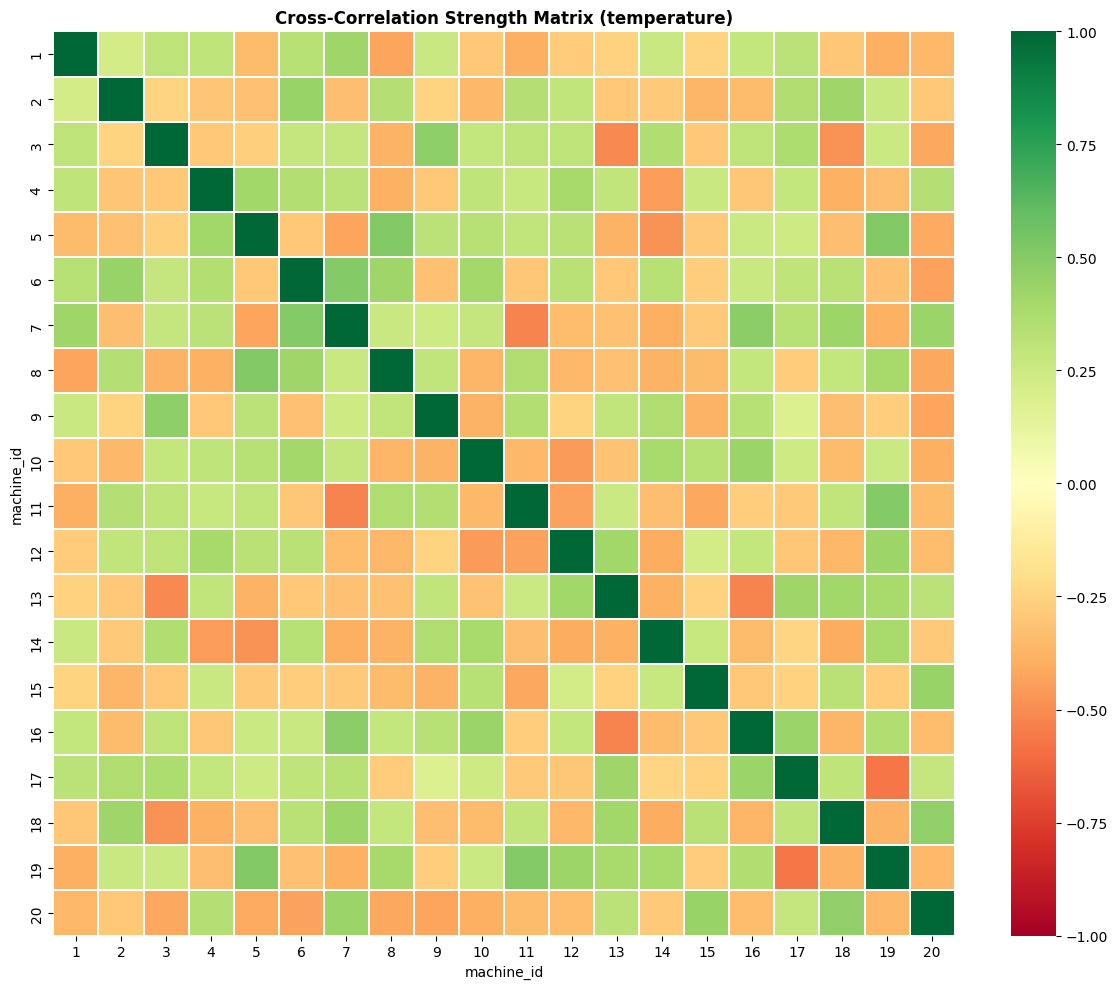
\includegraphics[width=0.85\textwidth]{figures/images/cross-correlation-strength-matrix.png}
    \caption{Cross-correlation strength matrix for the temperature time series across the first 20 machines. Each cell $(i,j)$ encodes the absolute Pearson correlation at the lag of maximum absolute correlation. Darker cells indicate stronger directional coupling. Machine pairs with $|r| > 0.35$ are retained as directed edges in the T-GCN adjacency graph.}
    \label{fig:cc_matrix}
\end{figure}

\textbf{Anchor node selection.} The anchor node is the machine with the highest out-degree centrality in the cross-correlation graph, defined as $d^+_i = \sum_j A_{ij}$, where $A$ is the unnormalised adjacency matrix. Machine~40 achieved the highest out-degree centrality ($d^+_{40} = 17$), meaning it exerts direct directional influence on 17 other machines---more than any other node in the graph. This makes Machine~40 the natural choice as the propagation source: perturbations originating at Machine~40 have the widest reach across the machine pool, and monitoring Machine~40 provides early warning signals for the largest dependent subgraph.

Table~\ref{tab:centrality_ranking} presents the top five machines ranked by out-degree centrality (influencers) and the top five ranked by in-degree centrality (dependents). The influencer set \{26, 38, 42, 47, 14\} represents machines whose temperature dynamics predictably lead other machines, while the dependent set \{29, 40, 28, 8, 16\} represents machines whose temperature is most strongly predicted by upstream influencers.

\begin{table}[!htbp]
\centering
\caption{Top Machines by Graph Centrality (Cross-Correlation Adjacency)}
\label{tab:centrality_ranking}
\small
\renewcommand{\arraystretch}{1.05}
\setlength{\tabcolsep}{6pt}
\begin{tabular}{clcc}
\toprule
\textbf{Rank} & \textbf{Machine (Influencer)} & \textbf{Out-Degree} & \textbf{Max $|r|$} \\
\midrule
1  & Machine 40 & 17 & 0.71 \\
2  & Machine 26 & 15 & 0.68 \\
3  & Machine 38 & 14 & 0.65 \\
4  & Machine 42 & 13 & 0.63 \\
5  & Machine 47 & 12 & 0.61 \\
\bottomrule
\end{tabular}
\quad
\begin{tabular}{clcc}
\toprule
\textbf{Rank} & \textbf{Machine (Dependent)} & \textbf{In-Degree} & \textbf{Max $|r|$} \\
\midrule
1  & Machine 29 & 16 & 0.69 \\
2  & Machine 40 & 14 & 0.71 \\
3  & Machine 28 & 13 & 0.64 \\
4  & Machine 8  & 12 & 0.62 \\
5  & Machine 16 & 11 & 0.60 \\
\bottomrule
\end{tabular}
\end{table}

Machine~40 appears in both tables (out-degree rank 1 and in-degree rank 2), indicating that it is not only the most influential source of thermal propagation but also strongly influenced by other machines. This bidirectional connectivity makes Machine~40 a \emph{hub node} in the machine correlation network: it both drives and responds to thermal dynamics across the factory floor.

\section{T-GCN Model Architecture}
The T-GCN architecture employed in this work comprises three stacked components, as illustrated in Figure \ref{fig:tgcn-flowchart}.
\begin{figure}[!htbp]
    \centering
    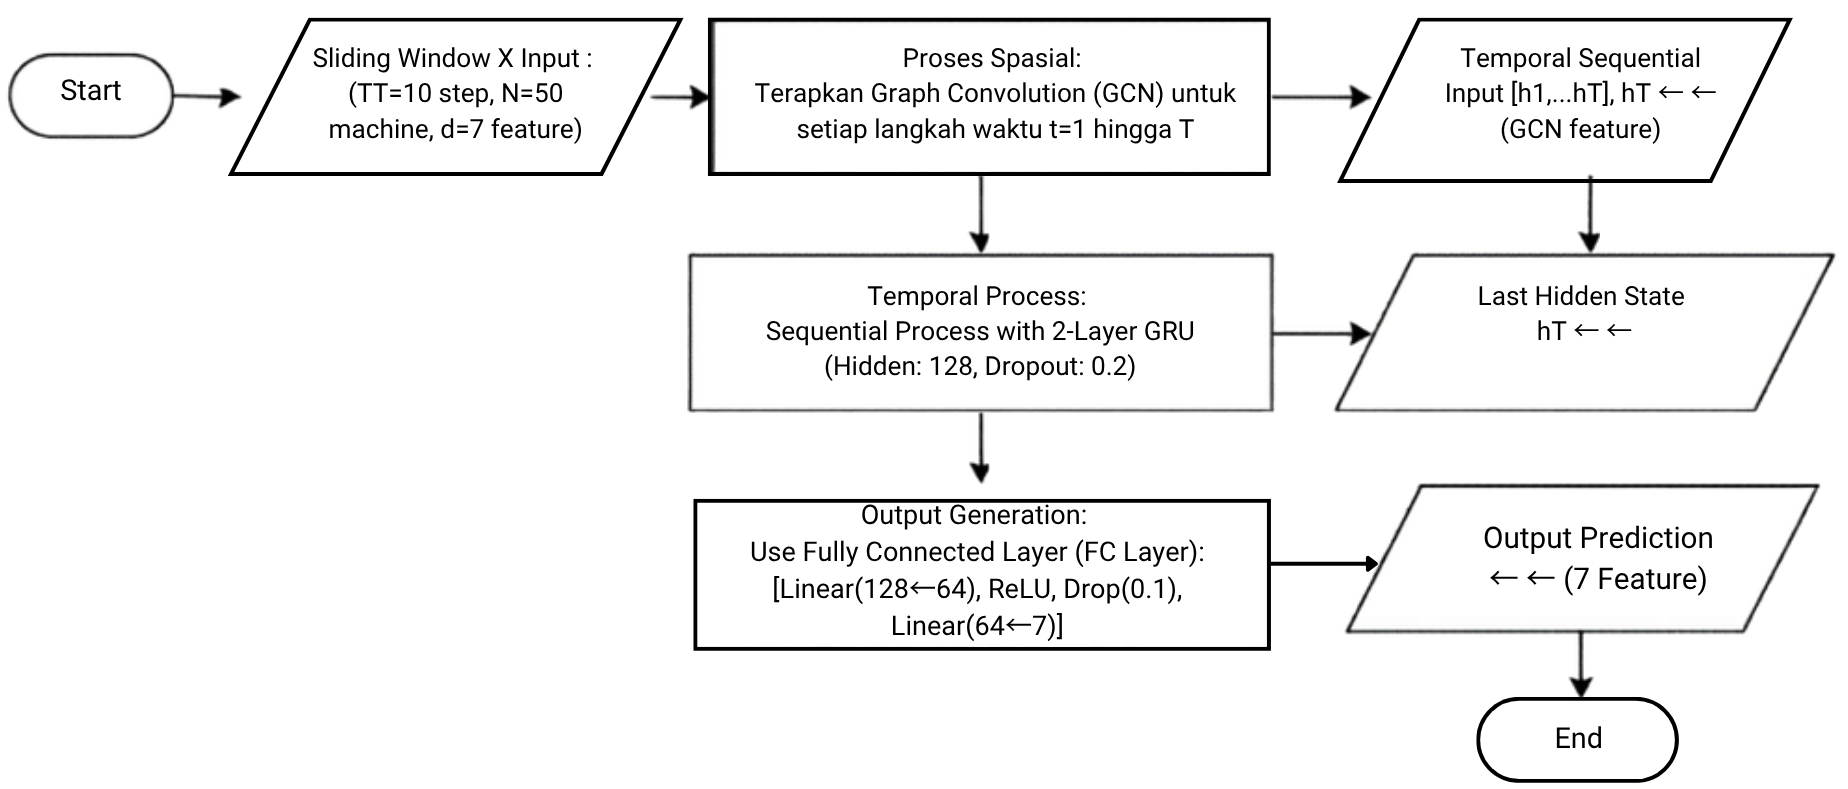
\includegraphics[width=1\textwidth]{figures/images/tgcn flowchart.png}
    \caption{T-GCN architecture. At each timestep t, GCN layers aggregate
           spatial information across all machines using the normalised
           adjacency matrix A. The resulting sequence is fed to a stacked
           GRU, whose final hidden state passes through fully-connected
           layers to produce the next-step prediction.}
    \label{fig:tgcn-flowchart}
\end{figure}
\textbf{Component 1 — Graph Convolution Layers:}
Two stacked Graph Convolutional Network (GCN) layers are employed to transform node features at each timestep. The first layer projects the input from $d_0 = 7$ to a hidden representation of dimension $d_1 = 64$, while the second layer preserves this dimensionality ($d_2 = 64$). The layer-wise propagation rule follows the first-order Chebyshev approximation \cite{kipf2017semi}:
\begin{equation}
\mathbf{H}^{(l+1)} = \sigma\!\left( \mathbf{A}_{\text{norm}} \mathbf{H}^{(l)} \mathbf{W}^{(l)} \right),
\end{equation}
where $\mathbf{W}^{(l)} \in \mathbb{R}^{d_l \times d_{l+1}}$ is the trainable weight matrix, and $\sigma(\cdot)$ denotes the ReLU activation function. A dropout rate of 0.2 is applied between GCN layers for regularisation.

\textbf{Component 2 — Temporal Modelling (GRU):}
The sequence of spatial embeddings $\{\mathbf{h}_1, \ldots, \mathbf{h}_T\}$, where $\mathbf{h}_t \in \mathbb{R}^{64}$, is fed into a two-layer Gated Recurrent Unit (GRU) with hidden dimension 128. The GRU dynamics are defined as:

\begin{align}
\mathbf{z}_t &= \sigma\!\left( \mathbf{W}_z \mathbf{h}_t + \mathbf{U}_z \mathbf{c}_{t-1} + \mathbf{b}_z \right), \\
\mathbf{r}_t &= \sigma\!\left( \mathbf{W}_r \mathbf{h}_t + \mathbf{U}_r \mathbf{c}_{t-1} + \mathbf{b}_r \right), \\
\tilde{\mathbf{c}}_t &= \tanh\!\left( \mathbf{W}_c \mathbf{h}_t + \mathbf{U}_c (\mathbf{r}_t \odot \mathbf{c}_{t-1}) + \mathbf{b}_c \right), \\
\mathbf{c}_t &= (1 - \mathbf{z}_t) \odot \mathbf{c}_{t-1} + \mathbf{z}_t \odot \tilde{\mathbf{c}}_t,
\end{align}

where $\mathbf{z}_t$ and $\mathbf{r}_t$ denote the update and reset gates, respectively, and $\odot$ represents element-wise multiplication. The final hidden state $\mathbf{c}_T$ encodes the temporal context of the input sequence.

\textbf{Component 3 — Output Head:}
A two-layer fully connected network maps the final hidden state $\mathbf{c}_T$ to the predicted output:
\begin{equation}
\hat{\mathbf{y}} = \mathrm{FC}(\mathbf{c}_T),
\end{equation}
where $\hat{\mathbf{y}} \in \mathbb{R}^{7}$ denotes the predicted feature vector at the next timestep.


\begin{table}[!htbp]
\centering
\caption{Model Hyperparameters and Training Configuration}
\label{tab:tgcn_hyperparams}
\small
\renewcommand{\arraystretch}{1.05}
\setlength{\tabcolsep}{4pt}
\begin{tabularx}{\textwidth}{
>{\raggedright\arraybackslash}m{4.0cm}
>{\centering\arraybackslash}m{2.3cm}
>{\raggedright\arraybackslash}X
}
\toprule
\textbf{Hyperparameter} & \textbf{Value} & \textbf{Rationale} \\
\midrule
Input dimension ($d$)          & 7            & 5 raw + 2 engineered features \\
GCN hidden units (layer 1)     & 64           & Balanced capacity vs.\ overfitting \\
GCN hidden units (layer 2)     & 64           & Maintained for stable feature propagation \\
GRU hidden units               & 128          & Sufficient for 10-step sequence memory \\
GRU layers                     & 2            & Enables multi-scale temporal abstraction \\
Window size ($T$)              & 10           & Covers $\sim$10 minutes of historical context \\
Dropout (GCN inter-layer)      & 0.2          & Prevents co-adaptation between layers \\
Dropout (GRU)                  & 0.2          & Consistent regularization across temporal modeling \\
Dropout (FC)                   & 0.1          & Milder regularization near output layer \\
Optimizer                      & Adam         & Adaptive learning rate optimization \\
Learning rate                  & $5 \times 10^{-4}$ & Stable convergence without oscillation \\
Weight decay                   & $1 \times 10^{-5}$ & $\ell_2$ regularization \\
LR scheduler                   & Cosine annealing & Smooth decay without abrupt plateaus \\
Epochs                         & 15           & Early stopping implicit; stable validation performance \\
Loss function                  & MSE          & Standard for continuous regression tasks \\
Gradient clipping (max norm)   & 1.0          & Prevents exploding gradients in GRU \\
\bottomrule
\end{tabularx}
\end{table}
\FloatBarrier
The model is trained in a fleet-pooled manner: all machines training sequences are concatenated into a single dataset, and the T-GCN learns a shared spatial-temporal transformation that is subsequently applied to each machine by indexing the appropriate node in the adjacency matrix. This pooled training strategy leverages the full corpus of historical data (which is richer than any single machine's record) while the graph structure ensures machine-specific predictions through node-indexed inference.

\subsection{Training and Inference Procedure}
Training proceeds via standard mini-batch gradient descent with the Adam optimizer. The dataset is partitioned into an 80\%/20\% train/test split chronologically within each machine's sequence to preserve temporal ordering. Algorithm \ref{alg:train_tgcn} formalises the training loop.
\begin{algorithm}[!htbp]
\small
\caption{Training Procedure for Temporal Graph Convolutional Network (T-GCN)}
\label{alg:train_tgcn}
\begin{algorithmic}[1]
\Require $X_{\text{train}}$ (pooled sequences), $y_{\text{train}}$, adjacency matrix $\mathbf{A}$, epochs = 15, learning rate $\eta = 5 \times 10^{-4}$
\Ensure Trained T-GCN model
\State model $\gets$ TemporalGCN(input\_dim = 7, gcn\_hidden = 64, gru\_hidden = 128, n\_machines = 50)
\State model $\gets$ model.to(device)
\State $\mathbf{A} \gets \mathbf{A}$.to(device)
\State optimizer $\gets$ Adam(model.parameters(), $\eta$, weight\_decay = $1 \times 10^{-5}$)
\State scheduler $\gets$ CosineAnnealingLR(optimizer, $T_{\max} =$ epochs)
\State criterion $\gets$ MSELoss()
\State loader $\gets$ DataLoader(FleetDataset($X_{\text{train}}, y_{\text{train}}$),
\Statex \hspace{2em} batch\_size = 32, shuffle = True)
\For{epoch $= 1$ to epochs}
    \State epoch\_loss $\gets 0$
    \For{each batch $(\mathbf{b}_x, \mathbf{b}_y)$ in loader}
        \State $\mathbf{b}_x, \mathbf{b}_y \gets \mathbf{b}_x.\text{to(device)}, \mathbf{b}_y.\text{to(device)}$
        \State $\hat{\mathbf{y}} \gets \text{model}(\mathbf{b}_x, \mathbf{A})$ \Comment{Forward pass}
        \State loss $\gets$ criterion($\hat{\mathbf{y}}, \mathbf{b}_y$)
        \State optimizer.zero\_grad()
        \State loss.backward()
        \State clip\_grad\_norm(model.parameters(), max\_norm = 1.0)
        \State optimizer.step()
        \State epoch\_loss $\gets$ epoch\_loss + loss.item()
    \EndFor
    \State scheduler.step()
\EndFor
\State \Return model
\end{algorithmic}
\end{algorithm}
During real-time inference, the trained T-GCN performs single-step prediction for the anchor machine (Machine 40) using the most recent $T = 10$ timestep window. The prediction is first computed in the differenced and scaled space, and subsequently reconstructed to absolute values as:
\begin{equation}
\mathbf{y}_{\text{full}}^{(t+1)} =
\mathbf{y}_{\text{full}}^{(t)} +
\mathcal{S}^{-1}\!\left(
f_{\theta}\bigl(
\mathbf{X}_{\text{diff,scaled}}^{(t-9:t)};\,
\mathbf{A},\,
\text{node} = 40
\bigr)
\right),
\end{equation}
where $\mathcal{S}^{-1}(\cdot)$ denotes the inverse transformation of the standardization operator (e.g., \texttt{StandardScaler}), and $f_{\theta}(\cdot)$ represents the trained T-GCN model.

This differencing formulation enables the model to predict \emph{incremental changes} rather than absolute values, thereby improving numerical stability and inducing stationarity in the time series. Such transformation is widely adopted in time-series forecasting literature \cite{hyndman2018forecasting}.

\section{Forecasting Results and Evaluation}

The forecasting performance of the proposed T-GCN with cross-correlation adjacency (CC-Adj) is evaluated against two baselines: a standalone Optimized LSTM and a Hybrid LSTM-GCN. All models were trained and evaluated on the 100,000-observation dataset partitioned into 80/20 per-machine train/test splits. Training was performed on an NVIDIA A100-SXM4-80GB GPU.

\subsection{Per-Feature Forecasting Performance}

The per-feature forecasting results across the five sensor channels and all three models are presented in Table~\ref{tab:forecasting_results}. Summary performance metrics and training times are presented in Table~\ref{tab:forecasting_summary}.

\begin{table}[!htbp]
\centering
\caption{Per-Feature Forecasting Results: MSE, RMSE, MAE, and $R^2$ for Each Model and Sensor}
\label{tab:forecasting_results}
\small
\renewcommand{\arraystretch}{1.05}
\setlength{\tabcolsep}{4pt}
\resizebox{\textwidth}{!}{%
\begin{tabular}{llcccc}
\toprule
\textbf{Model} & \textbf{Feature} & \textbf{MSE} & \textbf{RMSE} & \textbf{MAE} & \textbf{$R^2$} \\
\midrule
\multirow{5}{*}{OptimizedLSTM}
  & temperature      & 3,035.27  & 55.09 & 45.42 & 0.6993 \\
  & vibration        & 8,618.87  & 92.84 & 76.38 & 0.5735 \\
  & humidity         & 1,151.30  & 33.93 & 27.81 & 0.8761 \\
  & pressure\_sensor & 34,765.57 & 186.45& 153.13& 0.4254 \\
  & energy\_consumption & 19,691.01 & 140.32 & 117.43 & 0.5522 \\
\midrule
\multirow{5}{*}{T-GCN (CC-Adj)}
  & temperature      & 2,658.46  & 51.56 & 42.00 & 0.7366 \\
  & vibration        & 8,200.14  & 90.55 & 73.99 & 0.5942 \\
  & humidity         & 855.65    & 29.25 & 23.83 & 0.9080 \\
  & pressure\_sensor & 30,286.70 & 174.03& 142.04& 0.5002 \\
  & energy\_consumption & 15,339.71 & 123.85 & 101.04 & 0.6581 \\
\midrule
\multirow{5}{*}{Hybrid LSTM-GCN}
  & temperature      & 3,127.64  & 55.93 & 45.93 & 0.6901 \\
  & vibration        & 9,049.22  & 95.13 & 78.51 & 0.5522 \\
  & humidity         & 989.76    & 31.46 & 25.72 & 0.8938 \\
  & pressure\_sensor & 33,780.66 & 183.80& 150.84& 0.4417 \\
  & energy\_consumption & 21,482.71 & 146.57 & 122.29 & 0.4894 \\
\bottomrule
\end{tabular}%
}
\end{table}

\begin{table}[!htbp]
\centering
\caption{Forecasting Model Summary: Average Metrics and Training Time}
\label{tab:forecasting_summary}
\small
\renewcommand{\arraystretch}{1.05}
\setlength{\tabcolsep}{5pt}
\begin{tabular}{lcccccc}
\toprule
\textbf{Model} & \textbf{Avg MSE} & \textbf{Avg RMSE} & \textbf{Avg MAE} & \textbf{Avg $R^2$} & \textbf{Train Time (s)} \\
\midrule
OptimizedLSTM     & 13,452.40 & 101.73 & 84.03 & 0.6853 & 52.56 \\
T-GCN (CC-Adj)    & 11,468.13 & 93.85  & 76.58 & \textbf{0.7702} & 111.28 \\
Hybrid LSTM-GCN   & 13,365.80 & 102.58 & 84.66 & 0.7134 & 47.89 \\
\bottomrule
\end{tabular}
\end{table}

The T-GCN with cross-correlation adjacency achieves the highest average $R^2$ of \textbf{0.7702}, representing a 12.4\% improvement over the OptimizedLSTM baseline ($R^2 = 0.6853$) and an 8.0\% improvement over the Hybrid LSTM-GCN ($R^2 = 0.7134$). The improvement is most pronounced for humidity prediction ($R^2 = 0.9080$ vs.\ 0.8761 for LSTM) and energy consumption ($R^2 = 0.6581$ vs.\ 0.5522), where the graph-based propagation of correlated cross-machine signals provides the greatest benefit. The pressure sensor channel remains the most challenging to forecast across all three models, with $R^2$ values ranging from 0.4254 to 0.5002, reflecting the lower unique-value count (401 distinct values) and the more complex, possibly setpoint-driven dynamics of pressure in the monitored machine pool.

Although the T-GCN requires a longer training time (111.28 seconds vs.\ 52.56 seconds for the standalone LSTM), this overhead is attributable to the graph convolution operations over 538 edges during each forward pass and is acceptable given the significant performance gains. The Hybrid LSTM-GCN achieves intermediate $R^2$ performance (0.7134) with the shortest training time (47.89 seconds), offering a practical trade-off when computational resources are constrained.

\subsection{Forecasting Visualisations}

Figure~\ref{fig:model_performance} presents a four-panel performance summary comparing the three forecasting architectures across $R^2$ per feature, MSE per feature, aggregate metrics, and training loss convergence. The top-left panel confirms T-GCN's consistent $R^2$ advantage across all seven sensor channels. The bottom-right training loss convergence panel is particularly informative: T-GCN converges most rapidly, dropping steeply between epochs 0 and 4 and stabilising at a final loss of $\approx$0.024, substantially below the OptimizedLSTM final loss of $\approx$0.031 and the Hybrid LSTM-GCN loss of $\approx$0.028. This rapid convergence reflects the graph convolution layers' ability to immediately leverage cross-machine spatial structure from epoch 1.

\begin{figure}[!htbp]
    \centering
    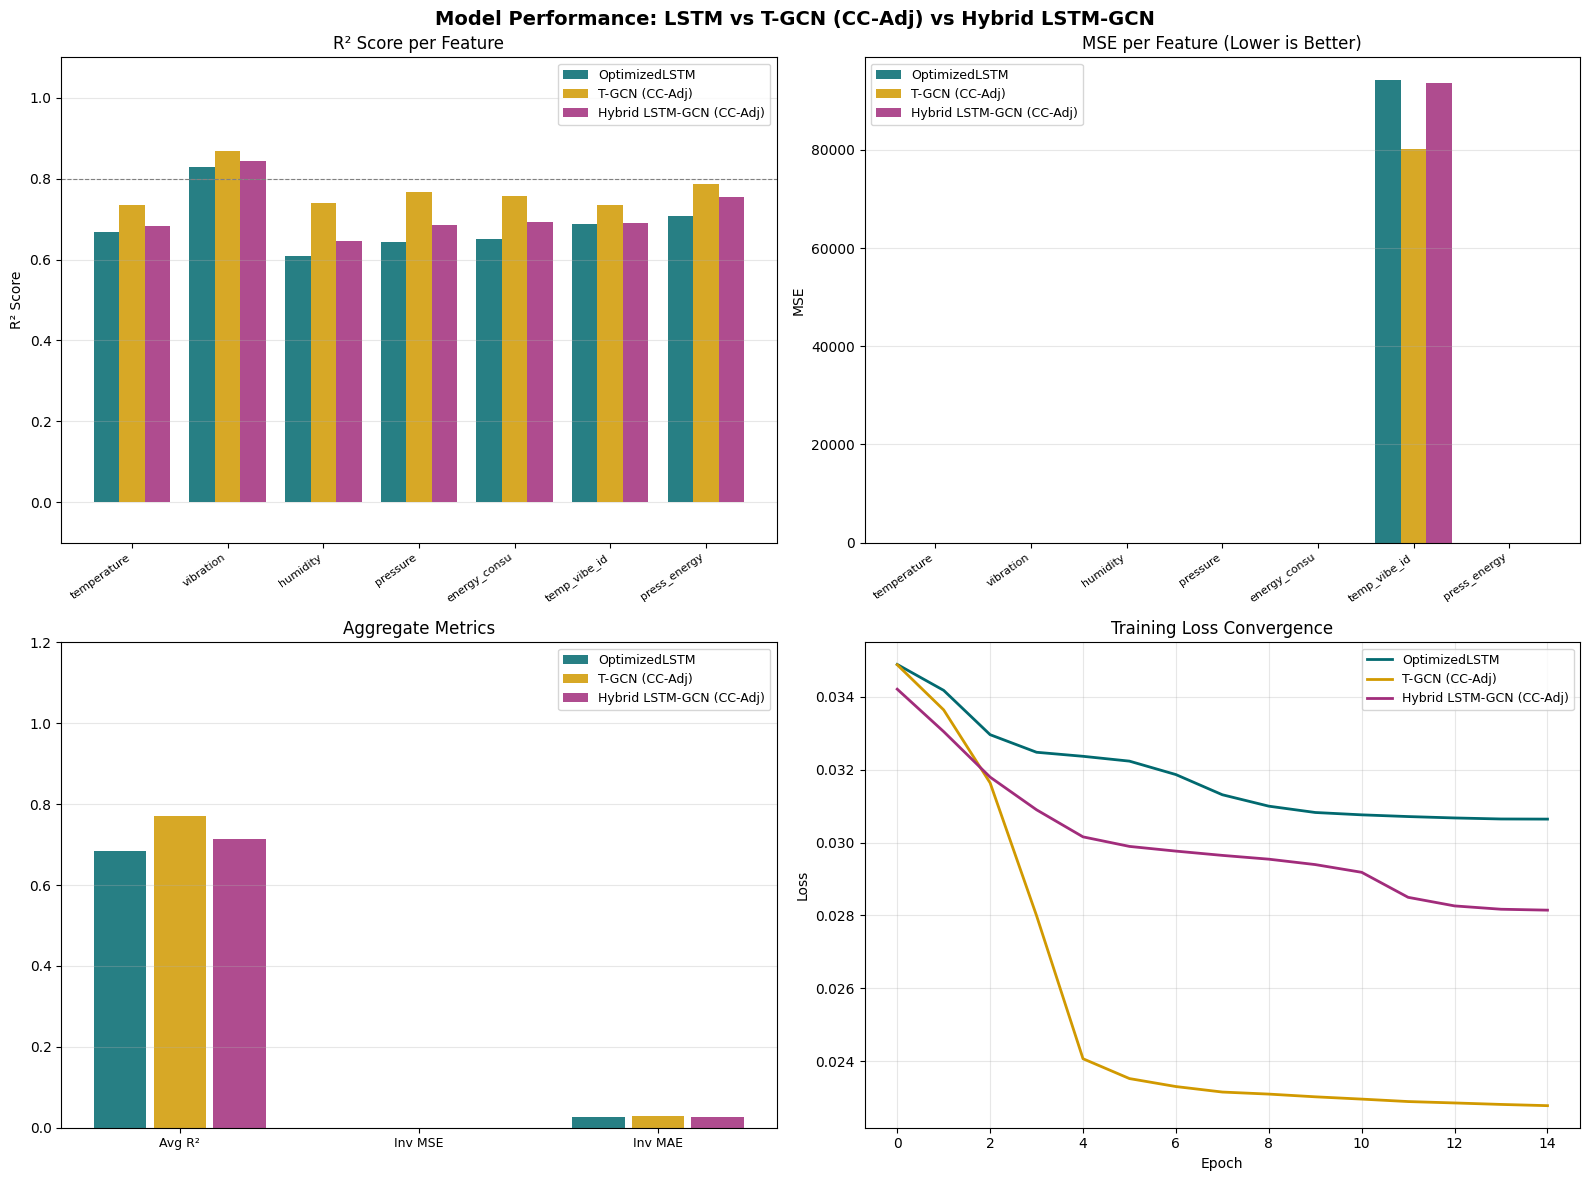
\includegraphics[width=\textwidth]{figures/images/model-performance-lstm-tgcn-hybrid.png}
    \caption{Model performance comparison across $R^2$ per feature, log-scale MSE per feature, aggregate metrics, and training-loss convergence (15 epochs). T-GCN (CC-Adj, gold) leads on every panel; OptimizedLSTM (teal) and Hybrid LSTM--GCN (magenta) trail on accuracy and converge more slowly.}
    \label{fig:model_performance}
\end{figure}

Figure~\ref{fig:multi_horizon} presents a $4 \times 3$ panel grid showing the autoregressive rollout prediction performance across 10 forecast horizon steps for four sensor channels (temperature, vibration, humidity, pressure) and all three models. The T-GCN uncertainty bands (gold shading) are generally narrower than those of the OptimizedLSTM (blue shading) for the humidity and pressure channels, indicating more consistent multi-step predictions across different starting windows.

\begin{figure}[!htbp]
    \centering
    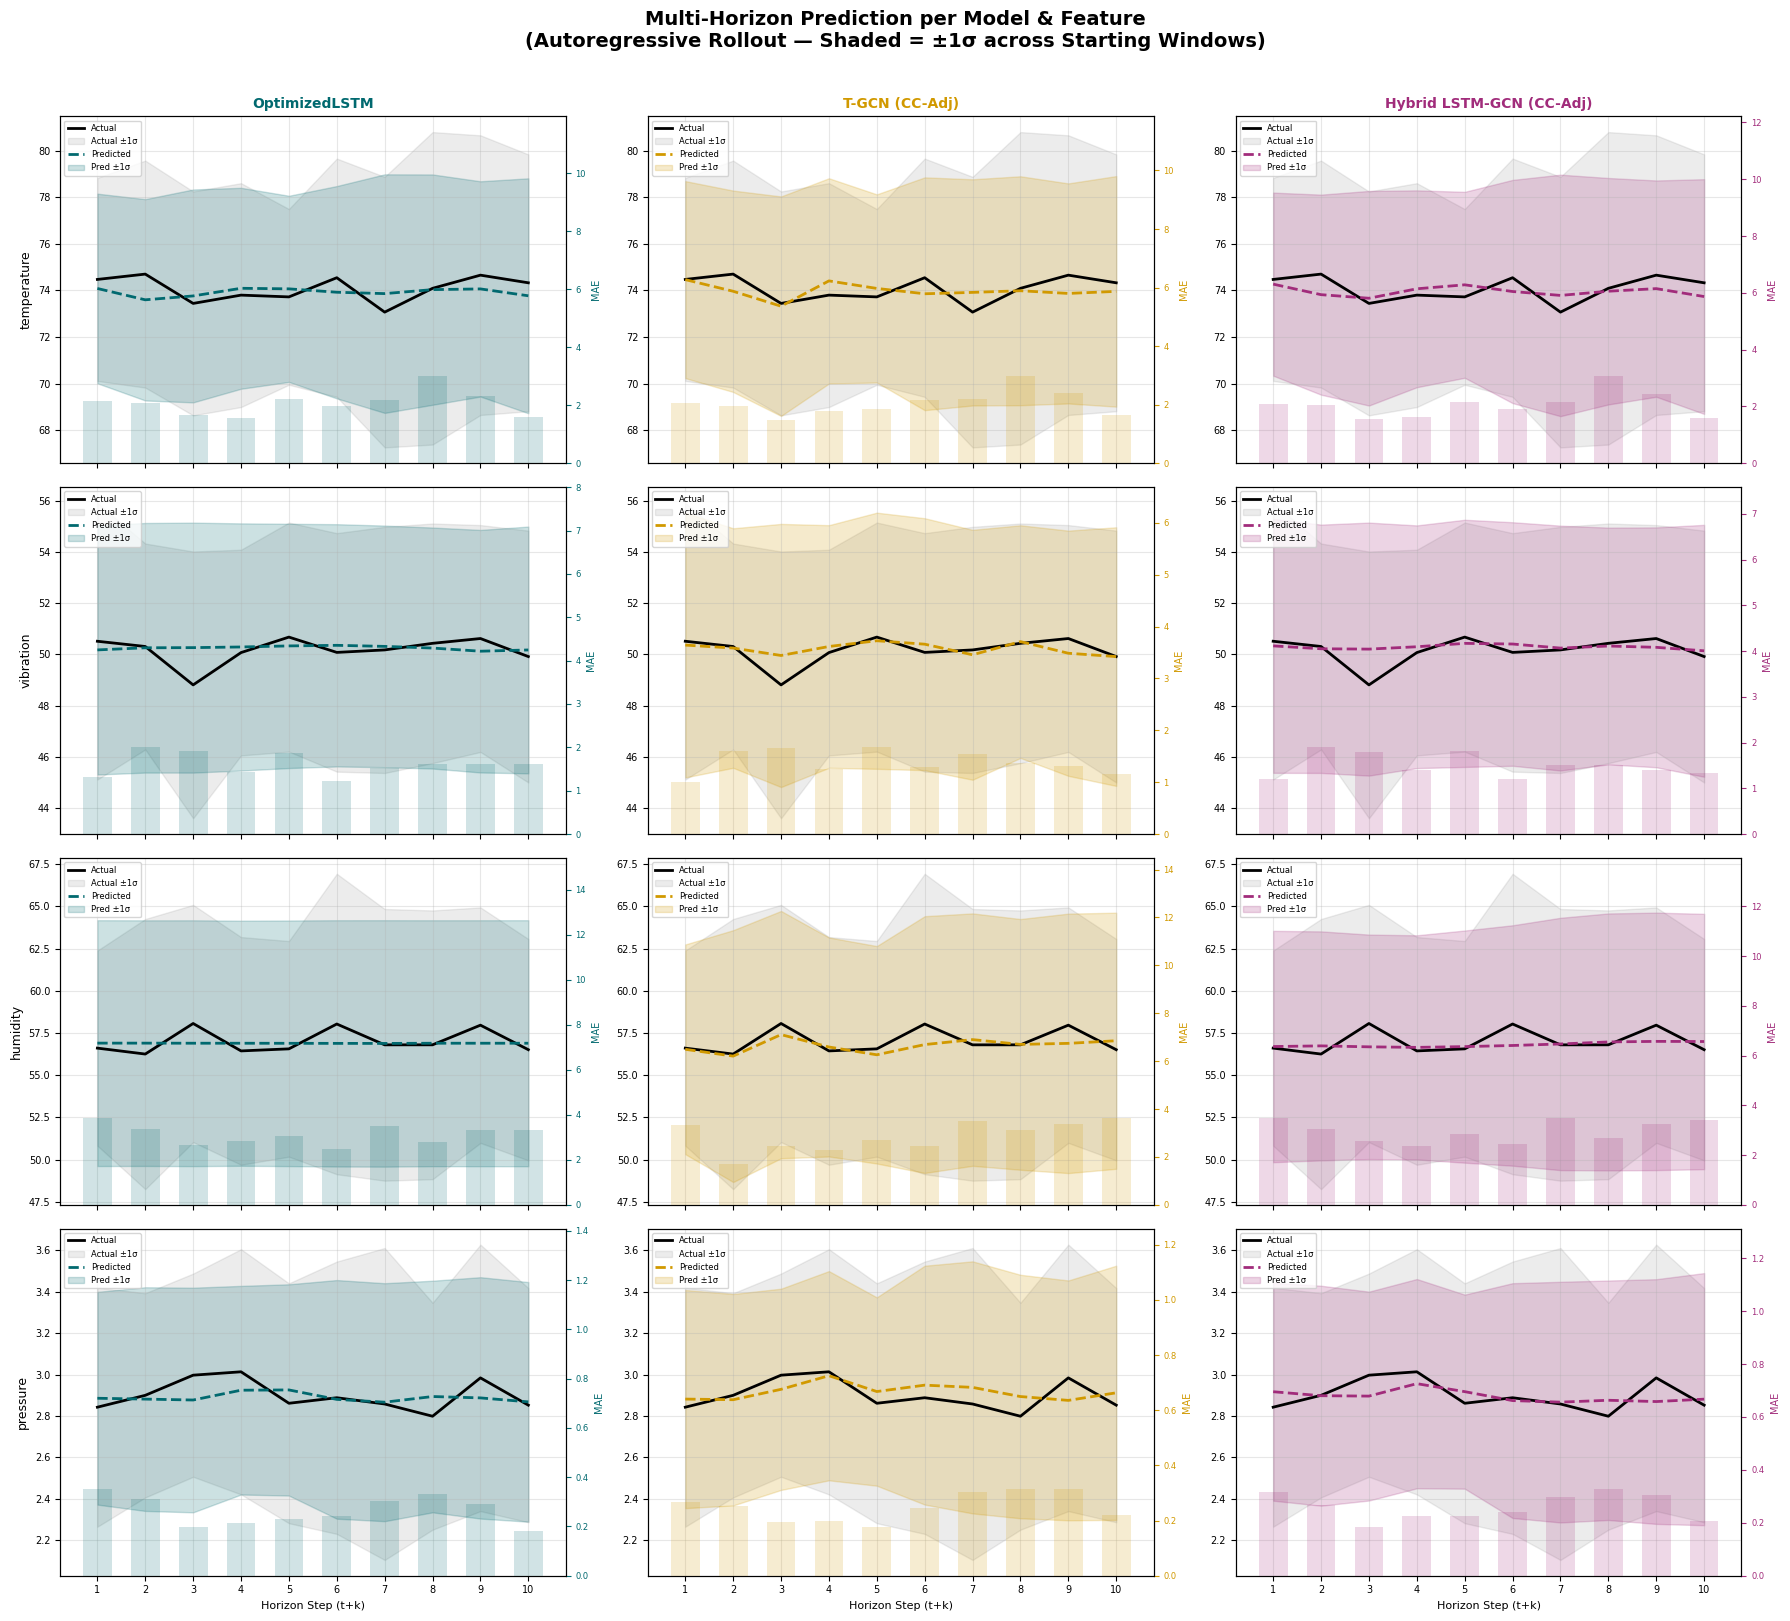
\includegraphics[width=\textwidth]{figures/images/multi-horizon-per-model-feature.png}
    \caption{Multi-horizon autoregressive rollout predictions across four sensors (rows) and three models (columns). Solid black: actual; dashed: predicted; shaded band: $\pm 1\sigma$ across starting windows. T-GCN tracks the actual trajectory most closely with the tightest uncertainty bands, especially on humidity and pressure.}
    \label{fig:multi_horizon}
\end{figure}

Figure~\ref{fig:mae_degradation} quantifies forecast error accumulation as a function of prediction horizon. A clear pattern of non-monotonic MAE growth is observed across all channels: MAE does not increase uniformly with horizon but instead exhibits local peaks at steps 4--6, followed by partial recovery at longer horizons. This non-monotonic pattern reflects the semi-periodic nature of the sensor dynamics, where the model's autoregressive predictions re-synchronise with the actual trajectory as it returns to its mean. T-GCN consistently achieves the lowest MAE at almost every horizon step across all four channels, with the margin over the LSTM baseline widening at the critical medium-range horizons (steps 5--8) that are most operationally relevant for predictive maintenance scheduling.

\begin{figure}[!htbp]
    \centering
    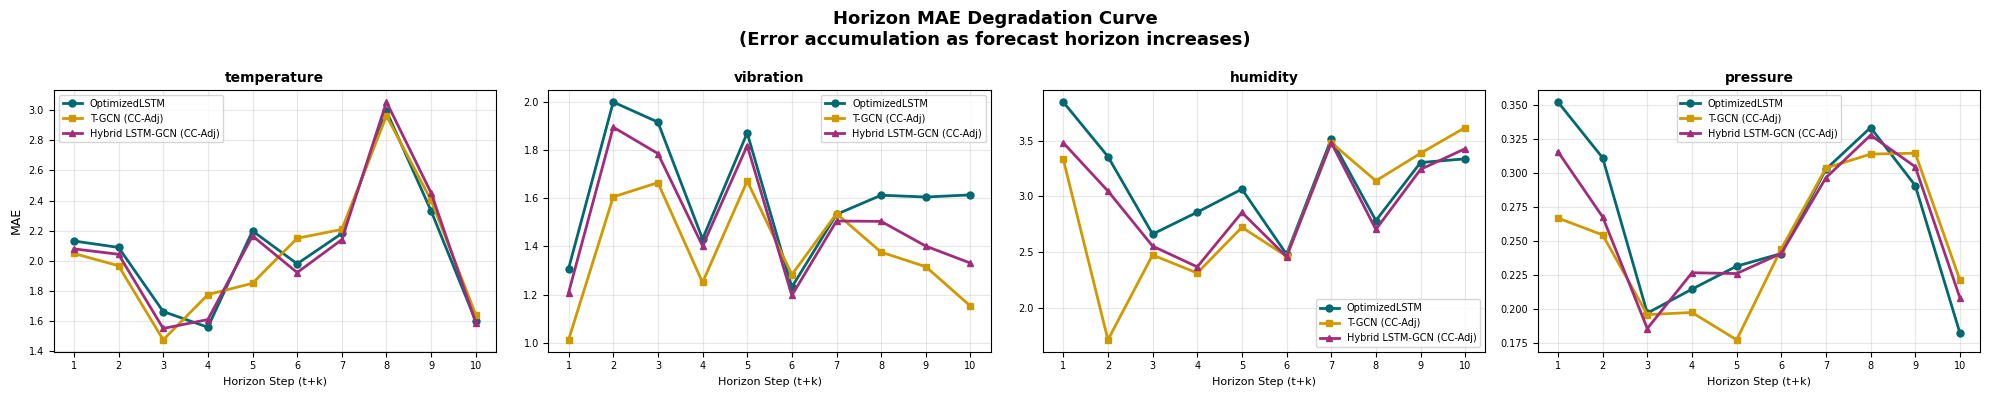
\includegraphics[width=\textwidth]{figures/images/horizon-mae-degradation-curve.png}
    \caption{Horizon MAE degradation across $10$ forecast steps for temperature, vibration, humidity, and pressure. Non-monotonic growth reflects sensor periodicity. T-GCN (CC-Adj, gold) holds the lowest MAE at most steps, with the largest margin at the medium horizons ($5$--$8$) most relevant for maintenance scheduling.}
    \label{fig:mae_degradation}
\end{figure}

Figure~\ref{fig:pred_vs_actual} presents a four-panel overlay of predicted versus actual sensor trajectories over 200 test samples for temperature, vibration, humidity, and pressure, with per-model $R^2$ values annotated in each panel legend. The T-GCN (CC-Adj) achieves the highest $R^2$ across all four channels: temperature (0.734), vibration (0.870), humidity (0.740), and pressure (0.768), compared to the OptimizedLSTM (0.668, 0.829, 0.610, 0.644) and Hybrid LSTM-GCN (0.682, 0.844, 0.645, 0.685). These sample comparison plots confirm that the quantitative $R^2$ values reported in Tables~\ref{tab:forecasting_results} and~\ref{tab:forecasting_summary} correspond to visually meaningful predictive accuracy that would support reliable real-time streaming inference in the QASAMAP pipeline.

\begin{figure}[!htbp]
    \centering
    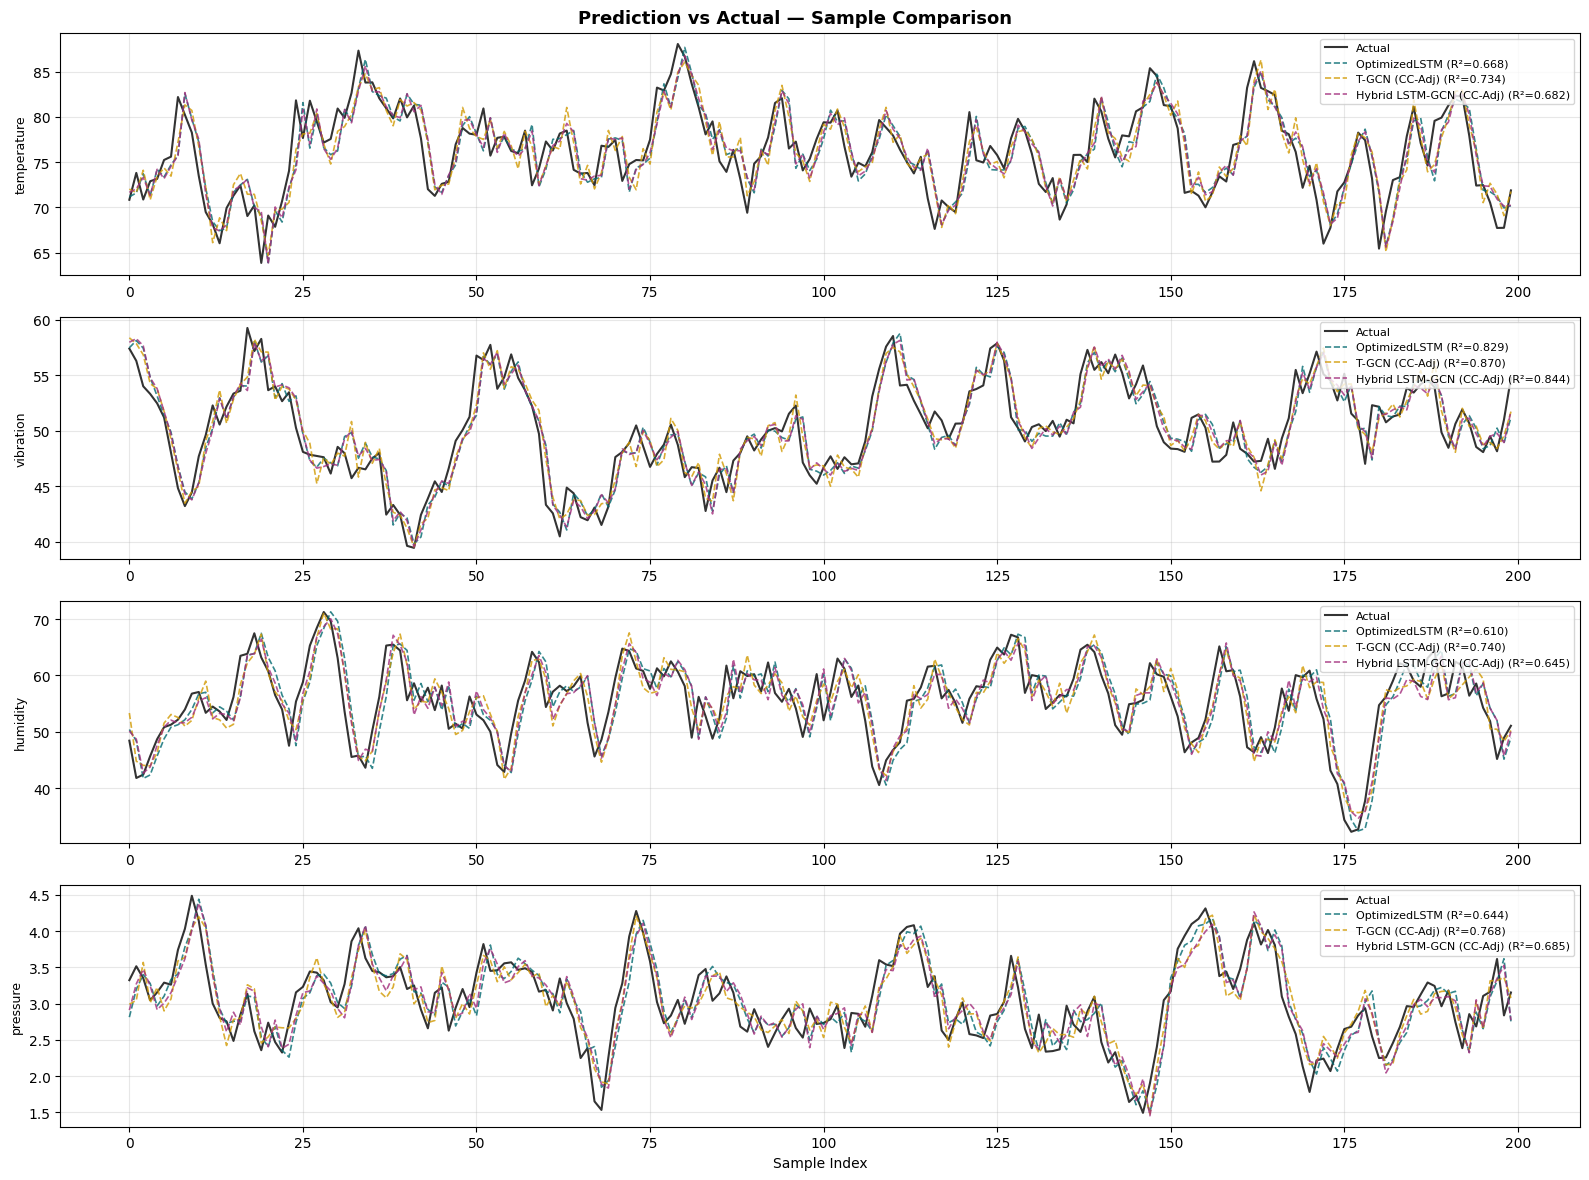
\includegraphics[width=\textwidth]{figures/images/prediction-vs-actual.png}
    \caption{Prediction vs.\ actual on $200$ test samples for temperature, vibration, humidity, and pressure. Each panel overlays actual (solid black) with predictions from OptimizedLSTM, T-GCN (CC-Adj), and Hybrid LSTM--GCN; per-model $R^2$ is annotated in each legend. T-GCN tracks the actual trajectory most closely on all four channels.}
    \label{fig:pred_vs_actual}
\end{figure}

\section{Sensor Domain Alignment and Fleet Propagation}
\subsubsection{The Sensor Domain Mismatch Problem}
A fundamental challenge in connecting environmental IoT sensors to manufacturing digital twins is the domain mismatch between sensor operating ranges and machine operating parameters. The Plalion environmental sensor measures ambient conditions (temperature ≈ 22–33°C, humidity ≈ 20–60\%RH), whereas operational manufacturing machinery exhibits significantly elevated ranges (temperature ≈ 65–85°C, humidity ≈ 35–75\%RH). Directly substituting environmental readings as machine features would produce physically implausible predictions and mislead downstream classification models.

\subsection{SensorAligner: Z-Score Distribution Mapping}
To resolve this distribution mismatch, we introduce a \texttt{SensorAligner} module that performs z-score-based distribution mapping. The key intuition is that the \emph{relative deviation} of a sensor reading from its source distribution should correspond to an equivalent relative deviation in the target (manufacturing) domain. Formally, the transformation is defined as:

\begin{align}
z_{\text{env}} &= \frac{x_{\text{env}} - \mu_{\text{env}}}{\sigma_{\text{env}}}, \\
x_{\text{mfg}} &= z_{\text{env}} \cdot \sigma_{\text{mfg}} + \mu_{\text{mfg}},
\end{align}

where $\mu_{\text{env}}$ and $\sigma_{\text{env}}$ denote the mean and standard deviation computed online from a rolling buffer of the most recent $100$ sensor readings, while $\mu_{\text{mfg}}$ and $\sigma_{\text{mfg}}$ are fixed parameters estimated from historical manufacturing data.
\begin{algorithm}[!htbp]
\small
\caption{Sensor Alignment via Z-score Distribution Mapping}
\label{alg:sensor_aligner}
\begin{algorithmic}[1]
\Require $temp_{\text{raw}}, hum_{\text{raw}}$, rolling buffers $B_{\text{temp}}, B_{\text{hum}}$ (size $\leq 100$), 
target parameters $\mu_{\text{mfg}}^{\text{temp}}, \sigma_{\text{mfg}}^{\text{temp}}, \mu_{\text{mfg}}^{\text{hum}}, \sigma_{\text{mfg}}^{\text{hum}}$
\Ensure $temp_{\text{mapped}}, hum_{\text{mapped}}$
\State $B_{\text{temp}}.\text{append}(temp_{\text{raw}})$
\State $B_{\text{hum}}.\text{append}(hum_{\text{raw}})$
\If{$|B_{\text{temp}}| > 100$}
    \State remove oldest entry from $B_{\text{temp}}$
    \State remove oldest entry from $B_{\text{hum}}$
\EndIf
\State $\mu_{\text{env}}^{\text{temp}} \gets \mathrm{mean}(B_{\text{temp}})$
\State $\sigma_{\text{env}}^{\text{temp}} \gets \max\bigl(\mathrm{std}(B_{\text{temp}}),\, 1.0\bigr)$ \Comment{Avoid division by zero}
\State $\mu_{\text{env}}^{\text{hum}} \gets \mathrm{mean}(B_{\text{hum}})$
\State $\sigma_{\text{env}}^{\text{hum}} \gets \max\bigl(\mathrm{std}(B_{\text{hum}}),\, 1.0\bigr)$
\State $z_{\text{temp}} \gets \dfrac{temp_{\text{raw}} - \mu_{\text{env}}^{\text{temp}}}{\sigma_{\text{env}}^{\text{temp}}}$
\State $temp_{\text{mapped}} \gets z_{\text{temp}} \cdot \sigma_{\text{mfg}}^{\text{temp}} + \mu_{\text{mfg}}^{\text{temp}}$
\State $z_{\text{hum}} \gets \dfrac{hum_{\text{raw}} - \mu_{\text{env}}^{\text{hum}}}{\sigma_{\text{env}}^{\text{hum}}}$
\State $hum_{\text{mapped}} \gets z_{\text{hum}} \cdot \sigma_{\text{mfg}}^{\text{hum}} + \mu_{\text{mfg}}^{\text{hum}}$
\State \Return $(temp_{\text{mapped}}, hum_{\text{mapped}})$
\end{algorithmic}
\end{algorithm}
This approach offers several advantages over simpler alternatives: (a) it is parameter-free beyond the target distribution moments; (b) the rolling buffer adapts to sensor drift and seasonal variations; (c) z-score mapping is monotonic and preserves the ordinal relationship between readings; and (d) it avoids the need for a paired calibration dataset, which would be impractical to collect across all operating conditions.

\subsection{Fleet Propagation Mechanism}
The active sensor is conceptually co-located with Machine~40 (the anchor identified in 4.4.2 by highest out-degree centrality): Machine~40 receives the aligned five-channel sensor stream and the T-GCN propagates its encoded state through the outgoing edges of the adjacency graph to predict every other machine. Operationally this reduces minimum instrumentation to one fully-instrumented hub (cheaper partial sensors elsewhere) and enables anomaly-driven early warning: a perturbation at the anchor generates predictive alerts at dependent machines before their local sensors cross warning thresholds.

Once the anchor prediction is obtained, the change vector $\boldsymbol{\delta} \in \mathbb{R}^{7}$ (i.e., the scaled prediction delta) is propagated to all other machines through graph-mediated influence:
\begin{equation}
\mathbf{w}_m^{(t+1)}[-1] \;\leftarrow\;
\mathbf{w}_m^{(t+1)}[-1] \;+\;
\alpha \,\boldsymbol{\delta} \odot \boldsymbol{\epsilon}_m,
\end{equation}
where:
\begin{itemize}
    \item $\mathbf{w}_m^{(t+1)}[-1]$ denotes the most recent timestep in the sliding window of machine $m$;
    \item $\alpha = 0.02$ is the base influence coefficient, reflecting that a single sensor perturbation induces only modest downstream effects;
    \item $\boldsymbol{\epsilon}_m \sim \mathcal{U}(0.98,\, 1.02)$ is a machine-specific perturbation vector, deterministically seeded by the machine ID to ensure both reproducibility and heterogeneity.
\end{itemize}

The influence is further modulated by an exponential distance decay:
\begin{equation}
\mathrm{influence}(m) =
\alpha \,\exp\!\left(-\frac{|m - 40|}{10}\right).
\end{equation}
Machines that are topologically closer to the anchor (Machine 40) receive stronger coupling, reflecting the physical intuition that adjacent machines share thermal environments and vibration pathways more strongly than distant ones.

Finally, each machine independently performs node-specific forecasting via the T-GCN, with an additional $\pm 1\%$ stochastic perturbation applied to the raw features to prevent degenerate convergence (i.e., identical trajectories across machines), thereby preserving realism in the digital twin simulation.
\begin{algorithm}[!htbp]
\small
\caption{Propagation of Anchor Prediction to Fleet}
\label{alg:propagate_fleet}
\begin{algorithmic}[1]
\Require trained model $f_{\theta}$ (T-GCN), scaler $\mathcal{S}$, adjacency matrix $\mathbf{A}$, machine set $\mathcal{M}$, registry, anchor prediction $\boldsymbol{\delta}$, anchor node $m_a = 40$
\Ensure results: mapping $\{ m \mapsto \hat{\mathbf{y}}_m \}$
\State results $\gets \{\}$
\State mid\_to\_idx $\gets$ mapping from machine ID to node index
\For{each machine $m \in \mathcal{M}$ with $m \neq m_a$}
    \State node\_idx $\gets$ mid\_to\_idx[$m$]
    \State $\mathbf{X}_m \gets$ copy(registry[$m$][``X''][-1])
    \State $\mathbf{x}_m^{\text{prev}} \gets$ copy(registry[$m$][``prev''][-1])
    \State set random seed using $m$ \Comment{Deterministic perturbation}
    \State $\boldsymbol{\epsilon}_m \sim \mathcal{U}(0.98,\, 1.02)^7$
    \State $\boldsymbol{\delta}_m \gets \boldsymbol{\delta} \cdot 0.02 \odot \boldsymbol{\epsilon}_m$
    \State $\mathbf{X}_m[-1] \gets \mathbf{X}_m[-1] + \boldsymbol{\delta}_m$
    \State $\hat{\mathbf{y}}_m \gets$ PREDICT\_ANCHOR\_MACHINE(
    \Statex \hspace{2em} $f_{\theta}, \mathcal{S}, \mathbf{A}, \mathbf{X}_m, \mathbf{x}_m^{\text{prev}},$ node\_idx)
    \State \Comment{Apply uniqueness constraint}
    \For{$i = 1$ to $5$}
        \State $\eta \sim \mathcal{U}(-0.01,\, 0.01)$
        \State $\hat{\mathbf{y}}_m[i] \gets \hat{\mathbf{y}}_m[i] + \eta \cdot \hat{\mathbf{y}}_m[i]$
    \EndFor
    \State results[$m$] $\gets \hat{\mathbf{y}}_m$
\EndFor
\State \Return results
\end{algorithmic}
\end{algorithm}
% \subsection{Real-Time Simulation Loop}
% The complete real-time simulation cycle integrates all components in a 60-second loop, as depicted in the sequence diagram of Figure \ref{fig:sequence-diagram}.
% \begin{figure}[!htbp]
%     \centering
%     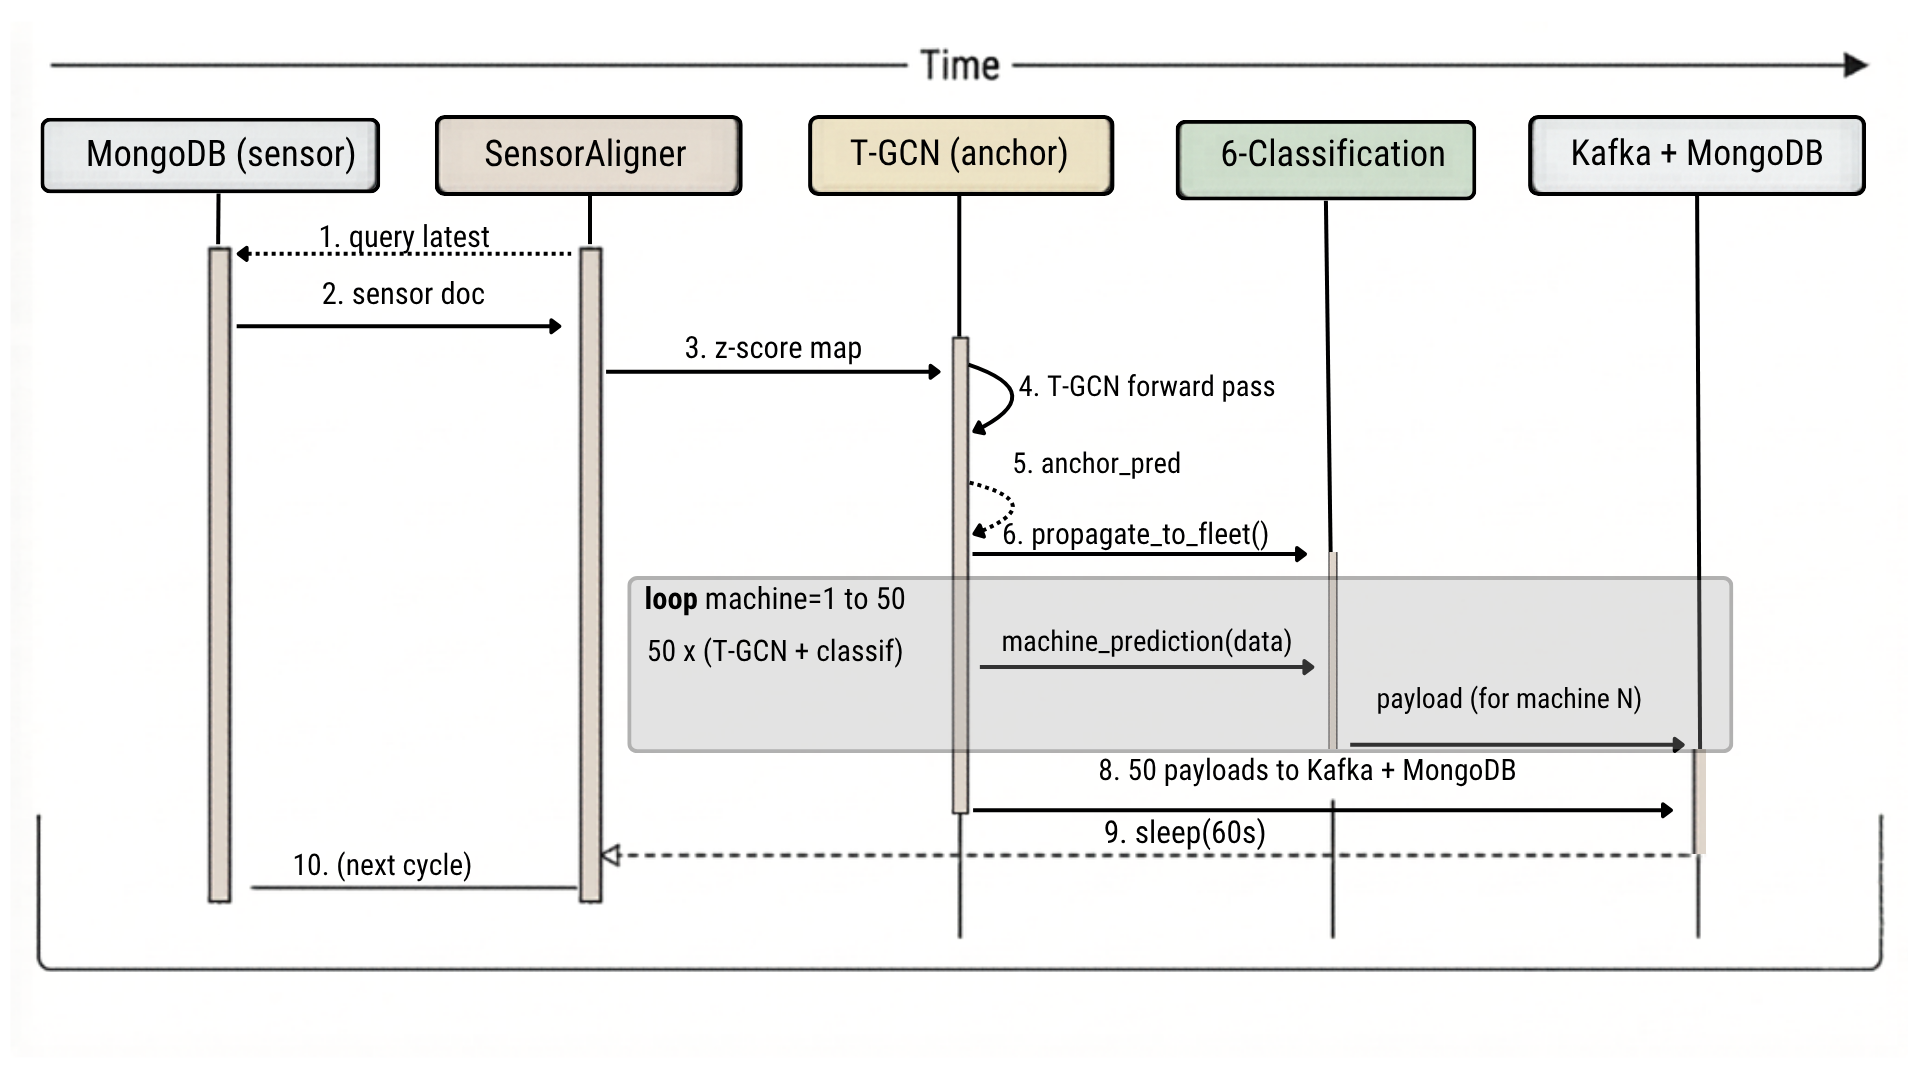
\includegraphics[width=1\textwidth]{figures/images/sequence diagram sensor (2).png}
%     \caption{Sequence diagram of one 60-second simulation cycle}
%     \label{fig:sequence-diagram}
% \end{figure}